\documentclass[10pt]{article}
\usepackage{icmlko}

\icmlmeta{IP 파운데이션 월드모델}{36}{상한은 두 개였다}{자기 상관을 올렸는데 전이가 따라오지 않았다 --- 노트 33 등식의 첫 반례와 그 원인}

\begin{document}

\twocolumn[
\icmlheader

\begin{abstract}
노트 35의 숙제부터 처리했다. 결측 패턴 누출을 네 도메인 스무 칸에서 기계적으로
검사했고 \textbf{전부 통과한다} --- 마스크만으로 라벨을 예측하면 팝업은 마스크
분산이 0이고, 아이돌 $-$0.158, 도서 $-$0.084로 음수이며, 게임만 $+$0.144인데
그 출처인 미디어 투입 축은 이미 파이프라인에서 빠져 있다. 그다음 본론으로
갔다. 노트 33·35가 확정한 대로 남은 지렛대는 대상 도메인의 자기 상관뿐인데,
지금까지 축을 다섯 개로 묶어 두었다. 그 제약은 \emph{공통 축에만} 필요하다 ---
고유 축은 정렬에 쓰이지 않으므로 도메인마다 개수도 종류도 달라도 된다. 그래서
버려 둔 정보를 고유 축으로 실었다. 팝업은 사람이 매긴 열 개 속성 중 다섯만 쓰고
있었다. 결과가 갈렸다 --- 자기 상관은 아이돌 0.651$\to$0.687, 게임
0.349$\to$0.388로 오르고 팝업 0.370$\to$0.232, 도서 0.203$\to$0.177로 내렸다.
그런데 \textbf{전이는 어느 경우에도 오르지 않았다}(9/12 유지, 게임만 8/12로
하락). \textbf{자기 상관이 올랐는데 전이가 안 오른 첫 사례다.} 원인을 팠다.
전이가 실제로 쓰는 2차원 인자 공간의 통과율을 재니 다섯 축에서는
\textbf{1.00--1.04로 무손실}인데 고유 축을 늘리면 아이돌 0.83, 도서 0.90으로
샌다. 고유 축 개수가 늘면 주성분이 그쪽으로 끌려가 정렬에 쓰는 공통 축 적재가
희석되는 것이다. $\lambda$는 겹침만 보정하고 \emph{개수}는 보정하지 않는다.
블록 정규화를 넣어 손실을 절반쯤 되돌렸지만(아이돌 0.554$\to$0.616) 다섯 축을
넘지 못했다. \textbf{전이의 상한은 두 개다} --- 대상의 자기 상관과, 정렬이
전달할 수 있는 몫. 지금까지는 전자가 구속했고 그래서 노트 33의 등식이 성립했다.
\end{abstract}
]

\section{먼저 결측 검사부터}

노트 35에서 도서의 판형 결측이 곧 전자책 여부였고 두 형식의 라벨이 열 배
달랐다. 그 검사는 손으로 했다. 여기서는 스무 칸(네 도메인 $\times$ 다섯 축)에
기계적으로 돌렸다 --- 마스크 자체가 라벨과 상관되는가.

\begin{figure}[t]
\centering

\includegraphics[width=\columnwidth]{figs/mask.pdf}
\caption{마스크만으로 라벨을 예측한 것과 축 값으로 예측한 것.}
\end{figure}

\begin{table}[t]
\centering\tsize
\caption{결측 패턴 누출 검사.}
\begin{tabular}{lrrl}
\toprule
도메인 & 마스크만 & 축 값만 & 판정 \\
\midrule
팝업 & 분산 0 & $+$0.370 & 전 축 100\% 태깅 \\
아이돌 & $-$0.158 & $+$0.435 & 음수 --- 신호 없음 \\
도서 & $-$0.084 & $+$0.226 & 음수 --- 신호 없음 \\
게임 & \textbf{$+$0.144} & $+$0.349 & 미디어 투입(38\%)에서 \\
\bottomrule
\end{tabular}
\end{table}

게임의 $+$0.144는 미디어 투입 마스크 하나에서 나오는데($r=+0.156$), 그 축은
관측률 38\%로 공통 축 문턱(60\%) 아래라 이미 파이프라인에서 빠져 있다.
\textbf{네 도메인 모두 통과다.} 팝업이 가장 걱정이었는데 --- 기획서에 안 적힌
것이 마스크 0이 되므로 ``큰 기획일수록 문서가 상세하다''면 같은 병이 생긴다 ---
실제로는 열 속성이 전부 태깅돼 있어 마스크에 분산이 없다.

\section{고유 축은 대응물이 필요 없다}

이제 본론이다. 노트 33·35가 확정했다 --- 전이 상관은 대상 자기 상관과 같고
($+$0.983) 남은 지렛대는 그것뿐이다.

그런데 지금까지 축을 다섯 개로 묶어 두었다. 도메인 간 대응물이 있어야 한다고
보았기 때문이다. 다시 보니 그 제약은 \emph{한쪽에만} 필요하다.

\begin{quote}\fontsize{9.5}{11.5}\selectfont
\textbf{공통 축}은 프로크루스테스 정렬에 쓰인다. 도메인 간 같은 물리량이어야
한다. 현재 타깃 폭과 굿즈 규모 둘뿐이다.\\[0.3em]
\textbf{고유 축}은 정렬에 쓰이지 않는다. 인자 공간을 만드는 데만 기여하고
$\lambda$로 축소된다. \textbf{도메인마다 개수도 종류도 달라도 된다.}
\end{quote}

즉 대응물이 없다는 이유로 버린 정보를 고유 축으로는 실을 수 있다. 팝업이 특히
아깝다 --- 사람이 기획서를 읽고 열 개 속성을 매겼는데 다섯만 쓰고 있었다.

\begin{table}[t]
\centering\tsize
\caption{추가한 고유 축과 라벨 상관. 라벨보다 나중에 쌓이는 값은 뺐다.}
\begin{tabular}{ll}
\toprule
도메인 & 추가 축 (라벨과 r) \\
\midrule
팝업 & 컬래버 강도 $+$0.170, 포토존 $+$0.136, \\
     & 체험 밀도 $+$0.081, IP 인지도 $+$0.051, \\
     & 계절 적합 $+$0.006 \\
아이돌 & 서바이벌 출신 $+$0.134, 사전 화제 $+$0.049, \\
     & 걸그룹 $-$0.007 \\
게임 & 기능 수 $+$0.293, 최소 RAM $+$0.218, \\
     & 연령 등급 $+$0.175, 가격 $+$0.095 \\
도서 & 무게 $-$0.086, 쪽수 $+$0.029 \\
\bottomrule
\end{tabular}
\end{table}

도서 리뷰 수와 별점은 뺐다 --- 판매지수와 함께 판매의 함수라 누출이다. 게임
DLC 수도 뺐다(노트 21에서 확인된 누출).

\section{자기 상관은 갈리고 전이는 안 움직였다}

\begin{figure}[t]
\centering

\includegraphics[width=\textwidth]{figs/own.pdf}
\caption{왼쪽 --- 고유 축 추가 전후 자기 상관. 오른쪽 --- 유의한 전이 방향.}
\end{figure}

\begin{table}[t]
\centering\tsize
\caption{고유 축을 더한 결과.}
\begin{tabular}{lrrr}
\toprule
추가 대상 & 자기 상관 & 유의 & 평균 이득 \\
\midrule
없음(기준) & --- & 9/12 & $+$0.0480 \\
팝업 & 0.370 $\to$ \textbf{0.232} & 9/12 & $+$0.0376 \\
아이돌 & 0.651 $\to$ \textbf{0.687} & 9/12 & $+$0.0486 \\
게임 & 0.349 $\to$ \textbf{0.388} & \textbf{8/12} & $+$0.0502 \\
도서 & 0.203 $\to$ \textbf{0.177} & 9/12 & $+$0.0459 \\
넷 모두 & --- & 9/12 & $+$0.0439 \\
\bottomrule
\end{tabular}
\end{table}

자기 상관이 오른 둘(아이돌, 게임)에서도 전이가 오르지 않는다. 게임은 오히려
유의가 9에서 8로 떨어진다.

\claimx{자기 상관이 올라도 전이가 따라오지 않는 경우가 있다. 노트 33의 등식은
축 구조가 고정된 상태에서만 성립한다.}{같은 축 구조 안에서 자기 상관만 올렸는데
전이가 안 오르는 사례가 나오면 등식 자체가 더 좁아야 한다.}

\paragraph{팝업이 왜 내려갔나}
커버리지 손실이 아니다 --- 확장 후에도 완전 케이스가 75/75로 그대로다. 추가한
다섯 중 셋은 라벨과 상관이 있다(컬래버 강도 $+$0.170, 포토존 $+$0.136). n$=$75에서
축을 다섯에서 열로 늘리면 능형 회귀가 잡음을 학습한다. 노트 11에서 팝업 피처
122개를 전부 주면 검정력이 사라진 것과 같은 현상이다.

\section{2차원이 병목인가 --- 아니었다}

전이는 2차원 인자 공간을 거친다. 고유 축을 늘려도 그 2차원에 실리지 않으면
전달되지 않을 것이다. 통과율을 쟀다.

\begin{figure}[t]
\centering
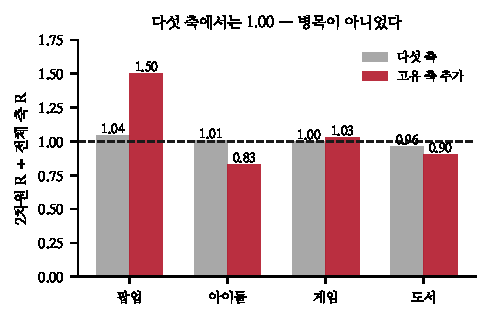
\includegraphics[width=\columnwidth]{figs/pass.pdf}
\caption{2차원 R을 전체 축 R로 나눈 값. 1이면 무손실이다.}
\end{figure}

\begin{table}[t]
\centering\tsize
\caption{인자 공간 통과율.}
\begin{tabular}{lrrr}
\toprule
도메인 & 전체 축 R & 2차원 R & 통과율 \\
\midrule
\multicolumn{4}{l}{\emph{다섯 축}} \\
\quad 팝업 & $+$0.370 & $+$0.385 & 1.04 \\
\quad 아이돌 & $+$0.651 & $+$0.656 & 1.01 \\
\quad 게임 & $+$0.349 & $+$0.349 & 1.00 \\
\quad 도서 & $+$0.203 & $+$0.195 & 0.96 \\
\midrule
\multicolumn{4}{l}{\emph{고유 축 추가}} \\
\quad 팝업 & $+$0.232 & $+$0.349 & 1.50 \\
\quad 아이돌 & $+$0.687 & $+$0.569 & \textbf{0.83} \\
\quad 게임 & $+$0.388 & $+$0.399 & 1.03 \\
\quad 도서 & $+$0.177 & $+$0.159 & \textbf{0.90} \\
\bottomrule
\end{tabular}
\end{table}

\textbf{다섯 축에서는 2차원이 병목이 아니다.} 통과율이 1.00--1.04로 사실상
무손실이다. 그러니 지금까지 K를 늘릴 이유가 없었다는 것도 확인된다.

고유 축을 늘리면 샌다. 아이돌은 전체 축 R이 0.651에서 0.687로 올랐는데 2차원
R은 0.656에서 0.569로 \emph{떨어졌다}.

\begin{figure}[t]
\centering

\includegraphics[width=\textwidth]{figs/two.pdf}
\caption{화살표가 전체 축 R의 상승을 표시한다. 2차원 R은 따라오지 않는다.}
\end{figure}

\section{$\lambda$가 개수를 보지 않는다}

원인은 인자 공간을 만드는 방식에 있다. 고유 축 블록은 $\lambda$배로 축소해
공유 블록과 함께 공분산 주성분을 뽑는다. 그런데 $\lambda_d$는 \emph{겹침}에서
유도한 값이지 \emph{개수}와 무관하다(노트 29).

고유 축이 다섯이면 그 블록의 분산 총량이 $\lambda^2\!\times\!5$가 되어 공유
블록(2)을 압도한다. 주성분이 고유 축 쪽으로 끌려가고, 정렬에 쓰는 공통 축
적재가 희석된다.

블록 전체의 분산을 공유 블록에 맞춘 뒤 $\lambda$를 거는 방식을 넣어 봤다.

\begin{table}[t]
\centering\tsize
\caption{고유 축 블록 정규화. 2차원 R 기준.}
\begin{tabular}{lrrr}
\toprule
도메인 & 다섯 축 & 확장(정규화 전) & 확장(정규화 후) \\
\midrule
팝업 & $+$0.373 & $+$0.348 & $+$0.348 \\
아이돌 & $+$0.656 & $+$0.554 & \textbf{$+$0.616} \\
게임 & $+$0.349 & \textbf{$+$0.402} & $+$0.380 \\
도서 & $+$0.195 & $+$0.159 & \textbf{$+$0.183} \\
\bottomrule
\end{tabular}
\end{table}

손실의 절반쯤을 되돌리지만 다섯 축을 넘지 못한다. 다섯 축 구조에 그대로 켜면
유의는 9/12로 같고 평균 이득이 $+$0.0480에서 $+$0.0469로 미세하게 나빠진다.
\textbf{채택하지 않고 기본값 끔으로 코드에만 남겼다.}

\section{상한이 두 개다}

\claimx{전이 성능은 두 상한 중 낮은 쪽에 묶인다 --- 대상 도메인의 자기 상관과,
정렬이 전달할 수 있는 몫. 지금까지 관측한 열두 셀은 전자가 구속하는 영역에
있었고, 그래서 노트 33의 등식이 성립했다.}{고유 축을 늘리지 않고 공통 축만
늘렸을 때도 전이가 자기 상관을 못 따라가면 이 이분법이 틀린 것이다.}

두 번째 상한은 공통 축 수의 함수다. 공통 축이 둘이므로 정렬은 $2\times K$
적재 행렬을 맞추고, 그것이 전달할 수 있는 구조에 한계가 있다. 고유 축을 아무리
쌓아도 그 관문을 통과하는 몫만 전달된다.

\begin{quote}\fontsize{9.5}{11.5}\selectfont
실무 규칙 --- \textbf{고유 축만 늘리는 것은 소용없다.} 자기 상관을 올리려면
공통 축을 늘려야 하고, 공통 축을 늘리려면 도메인 간에 같은 물리량을 새로
찾아야 한다. 측정 설계로 되돌아가는 문제다.
\end{quote}

노트 33의 마지막 문장 ``남은 일은 각 도메인에서 무엇을 어떻게 재느냐뿐이다''는
이제 더 구체적이다 --- \emph{네 도메인 모두에서 잴 수 있는} 새 물리량을 찾는
것이다.

\section{한계}

\begin{itemize}[leftmargin=1.1em,itemsep=0.15em]
\item 두 상한 가설을 직접 검정하지 못했다. 공통 축을 셋으로 늘려 전이가 오르는지
      봐야 하는데 네 도메인에 공통인 셋째 물리량을 아직 못 찾았다.
\item 팝업의 하락은 과적합으로 설명했지만 능형 강도를 바꿔 확인하지 않았다.
\item 고유 축을 개별적으로 넣지 않고 도메인마다 한꺼번에 넣었다. 좋은 것만
      골라 넣으면 다를 수 있고, 그 선택은 검정이 필요하다(노트 35의 교훈).
\item 블록 정규화 공식($\sqrt{|\text{공유}|/|\text{고유}|}$)은 유도한 것이 아니라
      분산을 맞추는 가장 단순한 형태를 고른 것이다.
\item 게임에서 자기 상관과 2차원 R이 모두 올랐는데 유의가 9에서 8로 떨어진
      이유를 보지 않았다. 정렬 쪽 변화로 보이지만 확인하지 않았다.
\end{itemize}

\section{다음}

\begin{enumerate}[leftmargin=1.3em,itemsep=0.15em]
\item 네 도메인 공통의 셋째 물리량 --- 두 상한 가설의 직접 검정이자 유일한 출구.
\item 팝업 고유 축을 하나씩 넣어 과적합 지점을 찾는다.
\item 게임 유의 하락(9$\to$8)의 정렬 쪽 원인.
\item 공통 축 수와 전달력의 관계를 합성 데이터로 확인한다.
\end{enumerate}

\vspace{0.6em}
\hrule height 0.3pt
\vspace{0.5em}
{\footnotesize
\textbf{참고문헌}\\[0.3em]
Schönemann, P. H. (1966). A generalized solution of the orthogonal Procrustes
problem. \emph{Psychometrika}, 31(1), 1--10.\\[0.15em]
Meredith, W. (1993). Measurement invariance, factor analysis and factorial
invariance. \emph{Psychometrika}, 58(4), 525--543.\\[0.15em]
Ben-David, S. et al. (2010). A theory of learning from different domains.
\emph{Machine Learning}, 79(1--2), 151--175.\\[0.15em]
Hastie, T., Tibshirani, R., Friedman, J. (2009). \emph{The Elements of
Statistical Learning}, 2nd ed. Springer.\\[0.15em]
Rubin, D. B. (1976). Inference and missing data. \emph{Biometrika}, 63(3), 581--592.
}

\end{document}
